\documentclass[10pt]{article}

\usepackage{amsmath}
\usepackage{fullpage}
\usepackage{array}
\usepackage{graphicx}
\usepackage{gensymb}
\usepackage{booktabs}
\usepackage{gensymb}
\usepackage{graphicx}
\usepackage{hyperref}
\hypersetup{colorlinks,urlcolor=blue}
\usepackage{mathtools}
\usepackage{dirtytalk}


\graphicspath{ {../Images/} }

\date{2014-6-22}
\pagestyle{empty}
\setlength{\parindent}{0pt}

\begin{document}
\begin{center}
\begin{Large}\textbf{Chapter: Special Relativity}\end{Large} \\
\smallskip
%\begin{large} Acceleration \end{large}
\end{center}
%%%%%%%
Objectives: proper frame of reference, space-time unification, relativistic/proper vectors
\section{Relativistic kinematics}
In the begning of the course, we studied the kinematical equations.  Let us consider the equation
\begin{equation}
  x(t)=ut+\frac{1}{2}at^2
\end{equation}
for a particle moving with constant acceleration $a$ with initial speed $u$.  For simplicity, we set $a=0$.  Thus the equation converts into
\begin{equation}
\label{kinem}
  x(t)=ut
\end{equation}
We can interpret equation \ref{kinem} as
\say{the displacement or \emph{space} of the particle as function of \emph{time}}.  According to this (Galilean) interpretation, time runs in the background (measured by the clocks) and spatial configurations \emph{depend} on the time.

Einstein's relativity aligns the \emph{space} and \emph{time} on the same footing.  According to this interpretation, ``spacetime'' is a single physical entity on which the physical events take place.  Furthermore, each physical quantity that we encountered earlier (distance, speed and momentum), has both space and time components!

Consider the spacetime graph of a shuttle `O' seen by Alice standing at the origin as shown. 
\begin{figure}[h]
\label{springhooke}
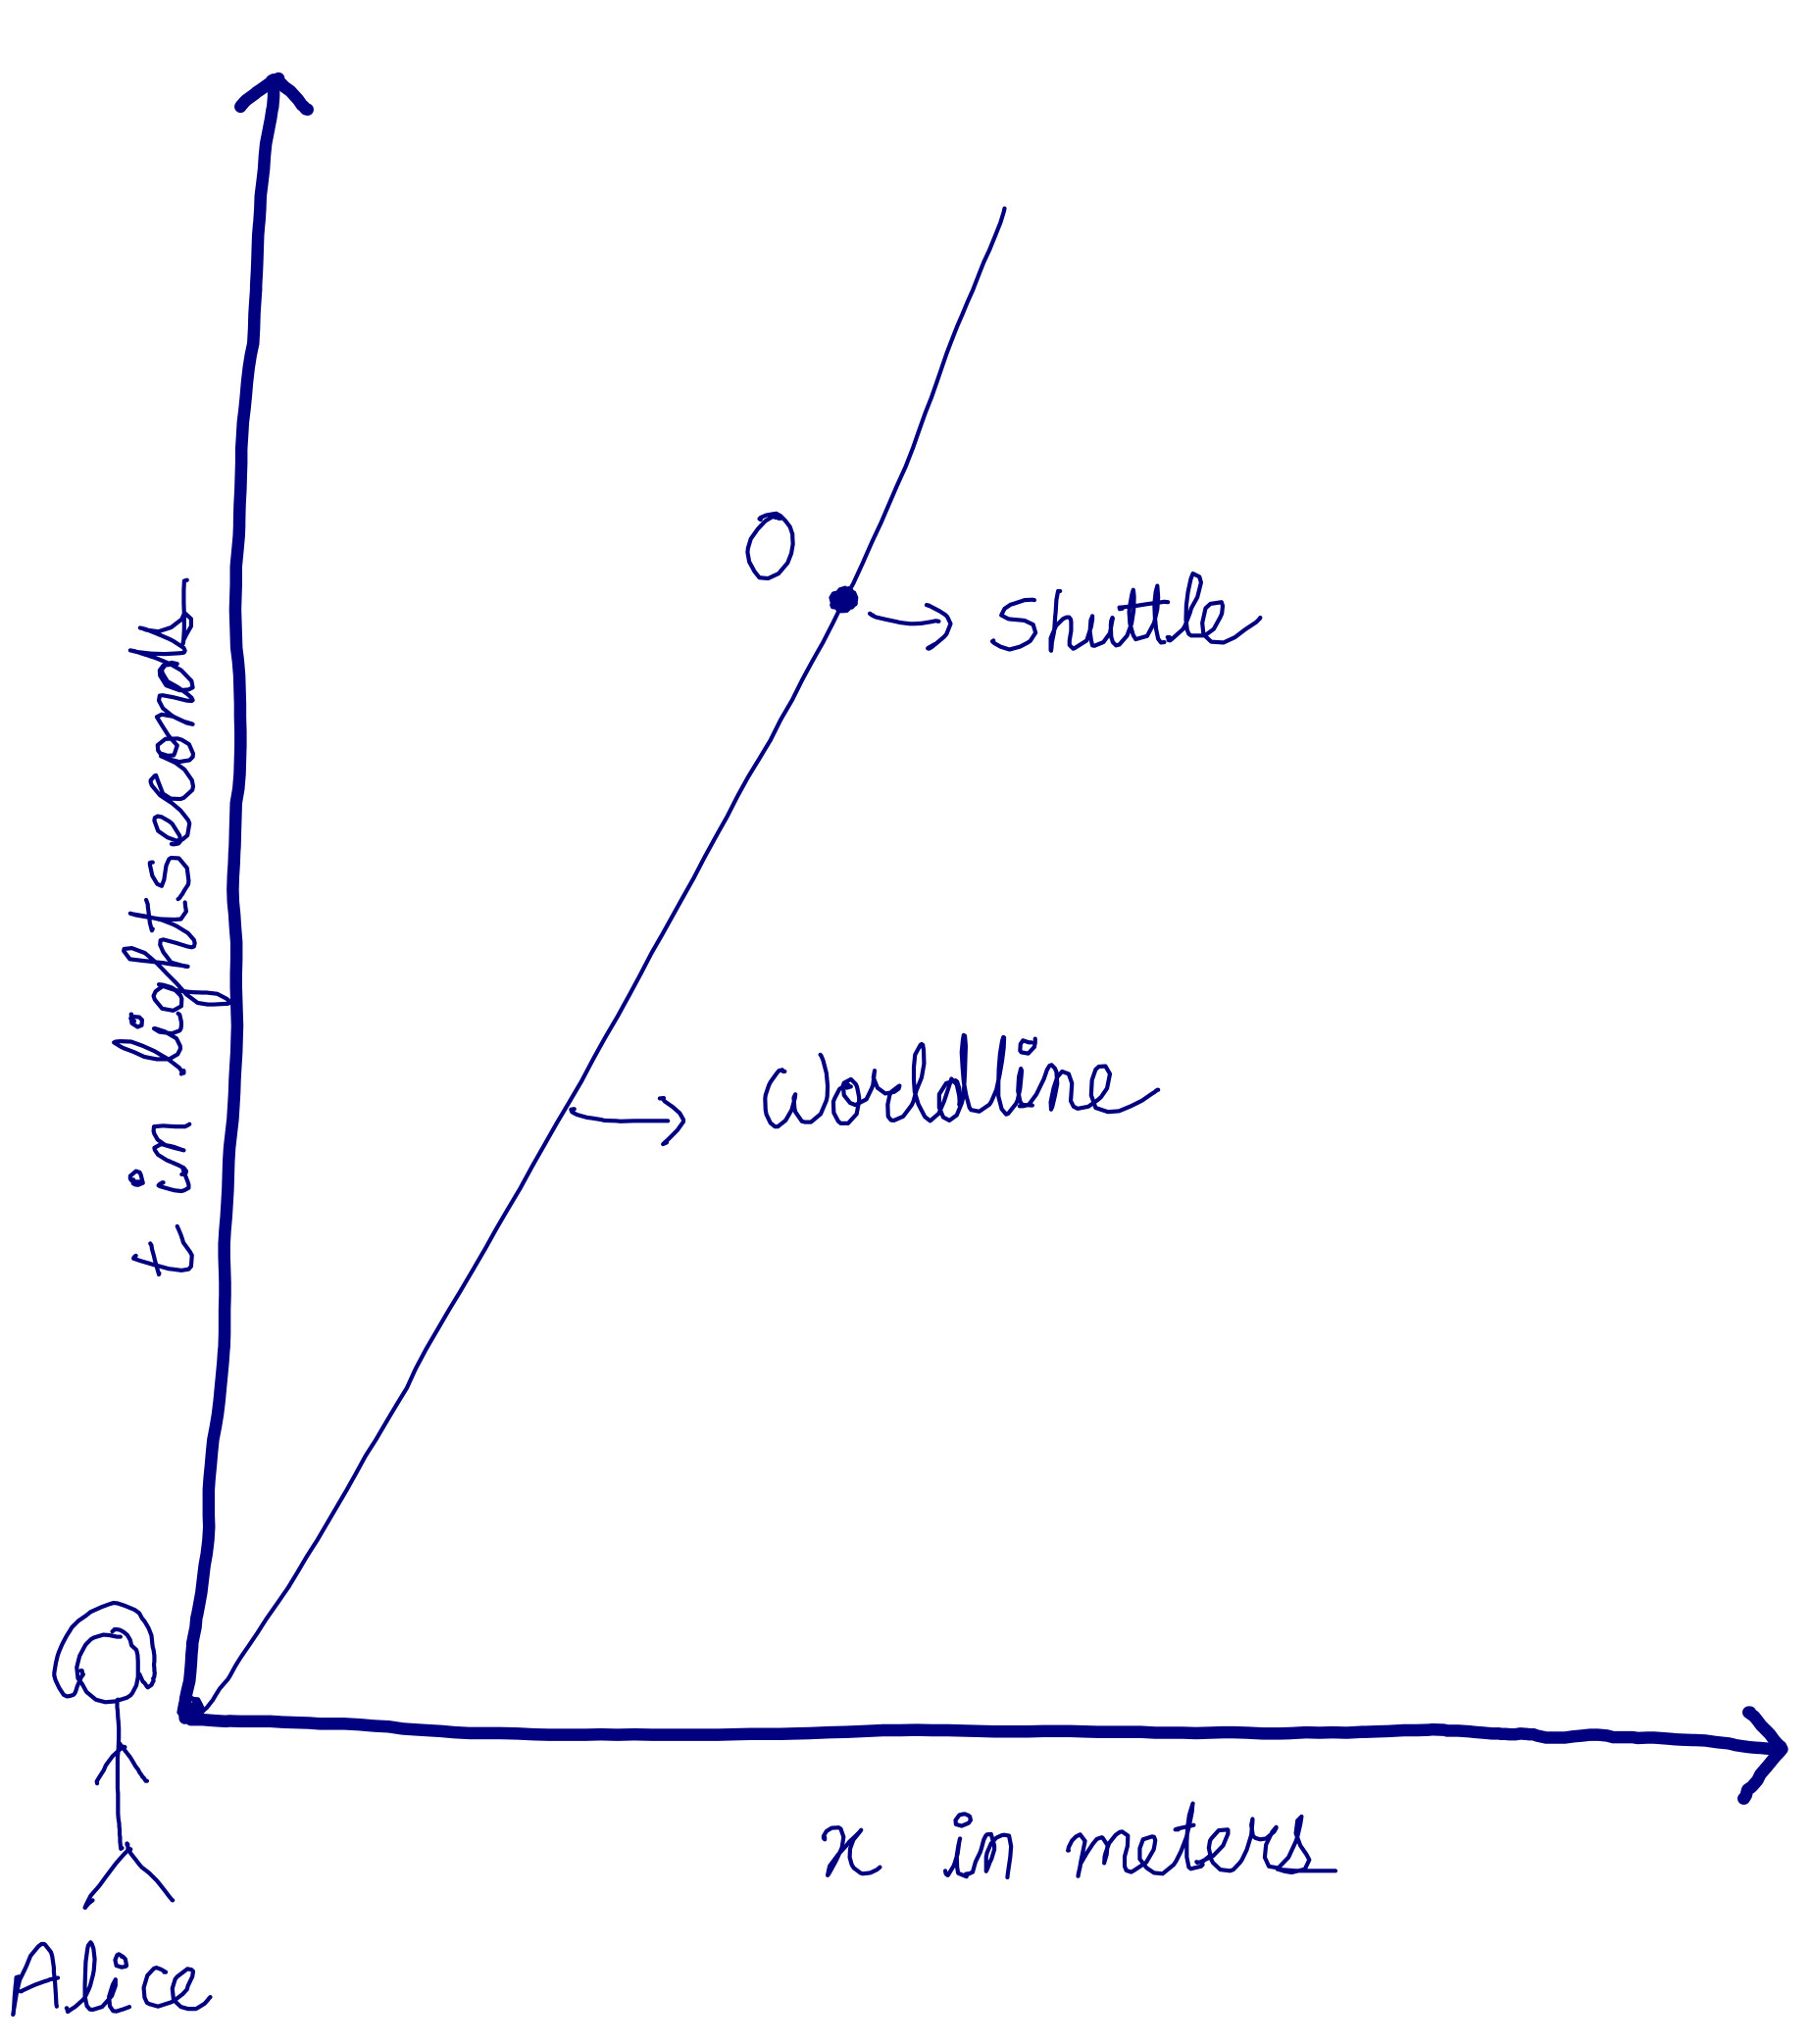
\includegraphics[scale=.4]{alicespacetime}
\centering
\caption{Spacetime graph with respect to Alice}
\centering
\end{figure}
We consider the functional dependance of spatial and temporal coordinates as observed by Alice as follows
\begin{equation}
  \begin{split}
    t&=t(\tau)\\
    x&=x(\tau)
  \end{split}
\end{equation}
where $\tau$ is called the proper time.  It is the time measured by the oberver Bob standing inside the shuttle `O' (in the exercises, you will draw the spacetime graph of the shuttle with respect to Bob).  According to Einstein's relativity, Bob's clock ($\tau$) ticks differently when compared with Alice's clock ($t$) \emph{in the spacetime graph drawn above}.

Now we will write the space and time components of the physical quantities we studied in the class. We will start with the distance.

\subsection{Proper displacement}
Earlier we just required the displacement to specify the state of the point particle.  Now we need \emph{both} displacement and time to specify the state of particle in terms of displacement vector
\begin{equation}
\label{dispvec}
  \vec{d}_p=t\hat{a}_t+x\hat{a}_x
\end{equation}
Here $\hat{a}_t$ and $\hat{a}_x$ are the unit vectors in time and space directions respectively.

Now recall when (with only spatial dimensions) $\vec{A}$ and $\vec{B}$ were orthogonal to each other and were oriented along $x$ and $y$ axis as shown
\begin{figure}[h]
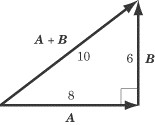
\includegraphics[scale=.5]{perp_vec}
\centering
\caption{Perpendicular vectors}
\centering
\end{figure}

Then the resultant vector $\vec{C}=A\hat{a}_x+B\hat{a}_y$ had the magnitude 
\begin{equation}
  |\vec{C}|=\sqrt{A^2+B^2}
\end{equation}  
where $A$ and $B$ were the magnitudes of $\vec{A}$ and $\vec{B}$ respectively.

For the proper (relativistic) vectors there is a minor difference.  The magnitude is given by 
\begin{equation}
  |\vec{d}_p|=\sqrt{t^2-x^2}
\end{equation}
Note the `$-$' sign instead of `$+$' sign.

\subsection{Proper speed}
In one spatial dimention, the speed is defined as $v=\Delta x/\Delta t$.  Now we define the proper \emph{space} speed as
\begin{equation}
\label{propspspeeddef}
  v_p^1=\frac{\Delta x}{\Delta \tau}=\frac{\text{displacement observed by Alice}}{\text{time elapsed in Bob's clock}}
\end{equation}
In exercises below you will show that
\begin{equation}
\label{propspspeed}
  v_p^1=\gamma\times v
\end{equation}
where $\gamma = \frac{\Delta t}{\Delta \tau}$.
Now we define proper \emph{time} speed as
\begin{equation}
  v_p^0=\frac{\Delta t}{\Delta \tau}=\gamma.
\end{equation}
Thus in our usual vector notation, we have proper speed vector given by
\begin{equation}
\label{propvel}
  \vec{v}_p=v_p^0\hat{a}_t+v_p^1\hat{a}_x
\end{equation}
In other words 
\begin{equation}
\vec{v}_p=\frac{\Delta \vec{d}_p}{\Delta \tau}.  
\end{equation}
where $\Delta \vec{d}_p$ is given by equation \ref{dispvec}.  The magnitude of the resultant is given by 
\begin{equation}
  ||\vec{v}_p|| = \sqrt{(v_p^0)^2-(v_p^1)^2}
\end{equation}

In the exercises you will show that for $||\vec{v}_p||=1$, 
\begin{equation}
\label{gammafind}
  \gamma = \frac{1}{\sqrt{1-v^2}}
\end{equation}
For $\gamma$ to be a real number $v<1$ (why?).

\subsection{Proper momentum}
\label{promom}
Recall that momentum $\vec{p}$ was defined as $m\times\vec{v}$.  Now we have proper momentum or energy-momentum as
\begin{equation}
\label{propmomdef}
  \vec{p}_p=m\vec{v}_p
\end{equation}
where $\vec{v}_p$ is given by equation \ref{propvel}.  In the exercises you will compute the $p_p^0$ and $p_p^1$.  According to Einstein's relativity, $p_p^0$ is energy and $p_p^1$ is the momentum associated with the shuttle as observed by Alice in her spacetime.

\section{Sample questions}
\begin{enumerate}
\item Draw the spacetime graph of the shuttle O with respect to Bob.
\vspace{250px}
\item Show that the equation \ref{propspspeed} can be obtained form the definition \ref{propspspeeddef}.
\vspace{250px}
\item From the statement $||\vec{v}_p||=1$ prove equation \ref{gammafind}.
\vspace{250px}
\item Time dilation: Assume that the shuttle O is moving with speed 0.5 m/s.  Find the time elapsed in Alice's clock, $\Delta t$, when Bob's clock ticks $\Delta \tau =1$ s. \\
Hint: Use the definition of proper time speed and the relation \ref{gammafind} you proved in the previous question.
\vspace{100px}\\
In the spacetime graph drawn by Alice, we can say that Bob ages \underline{\hspace{3cm}} (faster/slower) than Alice.  This relativistic phenomenon is called time dialation!
\item From the definition \ref{propmomdef} and equation \ref{propvel}, find the expressions for $p_p^0$ and $p_p^1$ in terms of $\gamma$, $m$ and $v$.
\vspace{250px}  
\item Dimensional analysis: In this chapter we have been neglecting the dimensions of physical quantities.  Let us rectify that in this exercise.  In the section \ref{promom}, we said that $p^0_p$ proportional to the Energy.  Let
\begin{equation} 
\label{einmc2}
\frac{E}{\text{constant}}=\text{constant}\times p^0_p  
\end{equation}
Find the SI units for the $\text{constant}$.
\vspace{100px}\\
Again, we consider the spacetime of Alice in which the shuttle is moving with the speed $.5$ m/s.  Write down the $\vec{p}_p$ (\ref{propmomdef}) of the shuttle.
\vspace{100px}\\
Finally write down the $\vec{p}_p$ of the shuttle with respect to Bob (who is moving with the shuttle).
\vspace{100px}\\
Let the constant = $c$ in equation \ref{einmc2}.  Find the energy $E$ of the shuttle with respect to Bob.  
\vspace{100px}\\
Voila! You just wrote Einstein's famous relativistic equation!
\end{enumerate}
\end{document}